\documentclass[12pt, a4paper, answers]{exam} % Lösungen
%\documentclass[12pt, addpoints, a4paper]{exam} % Ohne Lösungen
\newcommand{\myAuthor}{Constantin Lazari, Marco Wettstein}
\newcommand{\myTitle}{Übungen Informatik}
\newcommand{\mySubject}{Informatik III (2013)}
\newcommand{\myNumber}{4}

\usepackage[utf8]{inputenc}
\usepackage[pdftex]{graphicx} 
\usepackage{microtype}
\usepackage[pdfborder={0 0 0}, plainpages=false, pdfpagelabels]{hyperref} 
\usepackage[ngerman]{babel}
\usepackage[babel]{csquotes}
\usepackage{tabularx} 

\usepackage{tikz}
\usetikzlibrary{arrows,automata}
\usepackage{amsmath,amssymb,amsthm}

\usepackage{lmodern} %Type1-Schriftart fuer nicht-englische Texte
\hyphenation{eine einer eines} % Trennung von eine, einer, eines vermeiden
\usepackage{microtype}

\usepackage{color}
\usepackage{stmaryrd}
\usepackage{booktabs}


%% Listings %%%%%%%%%%%%%%%%%%%%%%%%%%%%%%%%%%%%%%%%%%%%%%%%%
%\usepackage{verbatim}
\usepackage{listings}
\lstloadlanguages{[LaTeX]TeX}
{\lstset{%
  basicstyle=\footnotesize\ttfamily,
  commentstyle=\slshape\color{green!50!black},
  keywordstyle=\bfseries\color{blue!50!black},
  identifierstyle=\color{blue},
  stringstyle=\color{orange},
  escapechar=\#,
  emphstyle=\color{red}}
}
{
  \lstset{%
    basicstyle=\ttfamily,
    keywordstyle=\bfseries,
    commentstyle=\itshape,
    escapechar=\#,
    emphstyle=\bfseries\color{red}
  }
}

\hypersetup{
	pdfauthor   = {\myAuthor},
	pdftitle    = {\myTitle},
	pdfsubject  = {\mySubject},
	pdfkeywords = {},
	pdfcreator  = {Kile},
	pdfproducer = {pdflatex},
	colorlinks 	= false
} 

\setlength{\parindent}{0em}
\setlength{\parskip}{0.75em}

%% Exam Settings
\pagestyle{headandfoot}
%\firstpageheader{Benutzer/innen im Umgang mit Informatikmitteln instruieren}{}{Lernkontrolle 1}
\firstpageheader{\mySubject}{}{Übung \myNumber}
\firstpageheadrule

%\runningheader{Benutzer/innen im Umgang mit Informatikmitteln instruieren}{}{Lernkontrolle 1}
\runningheader{\mySubject}{}{
\ifprintanswers
  Lösung Übung \myNumber
\else
  Übung \myNumber
\fi
}
\runningheadrule

\firstpagefooter{}{Seite \thepage\ von \numpages}{}
\firstpagefootrule

\runningfooter{}{Seite \thepage\ von \numpages}{}
\runningfootrule

\pointsinrightmargin
\pointpoints{Punkt}{Punkte}
\bonuspointpoints{Bonuspunkt}{Bonuspunkte}
\renewcommand{\solutiontitle}{\noindent\textbf{Lösung:}\par\noindent}

\CorrectChoiceEmphasis{\bfseries}
\renewcommand\choicelabel{$\boxempty$}

\begin{document}
	\begin{tabularx}{\textwidth}{Xr}
	\myAuthor & \today\\
	\end{tabularx}
  %% Lernkontrolle einbinden
	\begin{questions}
	\question
Die Zugriffszeiten unterschiedlicher Speicherarten beeinflussen erheblich die Leistung aktueller Computer bzw. Prozessoren.
\begin{parts}
\part
Recherchieren Sie aktuellen Werte für die Zugriffszeiten in Rechnern (Lesen und Schreiben) für:
\begin{itemize}
	\item SRAM (1st-Level-Cache)
	\item DRAM (Arbeitsspeicher)
	\item Festplatten (Massenspeicher) und 
	\item Solid State Disks (als Massenspeicher)
\end{itemize}
(Bitte mit Quellenangabe belegen)


\begin{solutionordottedlines}[2cm]
\begin{center}
\begin{tabular}{p{4cm}rp{3cm}}
	\toprule
	\multicolumn{1}{c}{\textbf{Speicher}} & \multicolumn{1}{c}{\textbf{Zugriffszeit}} & \multicolumn{1}{c}{\textbf{Quelle}}\\
	\midrule
	SRAM & 0.5 ns & \href{http://surana.wordpress.com/2009/01/01/numbers-everyone-should-know/}{wordpress.com}\\\hline
	DRAM & 10 -- 15 ns & \href{http://en.wikipedia.org/wiki/DDR3_SDRAM}{wikipedia.org}\\\hline
	Festplatte (HGST Ultrastar 7K3000 3 TB) & S: 5000 ns, L: 9000 ns & \href{http://www.chip.de/artikel/HGST-Ultrastar-7K3000-3-TB-HUA723030ALA640-SATA-Festplatte-3-5-Zoll-Test_63041861.html}{chip.de}\\\hline 
	SSD (Samsung SSD 840 EVO 1 TB) &  S: 23 ns, L: 31 ns & \href{http://www.chip.de/artikel/Samsung-840-EVO-1-TB-MZ-7TE1T0BW-SSD-Test_63269603.html}{chip.de}\\
	\bottomrule
\end{tabular}
\end{center}
\textit{S: schreiben, L: lesen}\\
Man stellt fest: Schreiben geht schneller als lesen!\\
Anmerkung: Im PDF sind die Links anklickbar und führen auf den Artikel.
\end{solutionordottedlines}
%%% Next subquestion

\part
Was sind die Vorteile und Nachteile der DDR(x)-SDRAM
Speicherbausteine (x steht für leer, 2
und 3) gegenüber klassischen DRAM-Bausteinen?
\begin{solutionordottedlines}[2cm]
\begin{description}
	\item [DDR-SDRAM] Datenbit wird bei auf und absteigender Flanke des Takt\-signals übertragen, statt nur bei einer Flanke wie beim SDRAM
	\begin{itemize}
		\item [$+$] theoretisch doppelte Datenrate
		\item [$+$] niedrige Betriebsspannung/geringer Stromverbrauch
		\item [$-$] Anzahl zusammenhängender Daten bei einer Anfrage muss mindestens so lang sein wie die doppelte Busbreite, ansonsten kann Geschwindigkeitsvorteil nicht erreicht werden
		\item [$-$] Address- und Steuersignale werden nur bei einer Taktflanke über\-tragen
 	\end{itemize}
	\item [DDR2] Vierfach-Prefetch statt zweifach
	\item [DDR3] Achfach-Prefetch statt zweifach
\end{description}

\end{solutionordottedlines}
%%% Next subquestion

\end{parts}
	\pagebreak
\question
Durch eine Speicherhierarchie soll der Benutzer sehr grossen Speicher zu sehr günstigen Kosten (virtuell) nutzen können.

Geben
Sie die aktuellen Grössenordnungen für:
\begin{itemize}
	\item die Kosten pro MB,
	\item die Zugriffgeschwindigkeit auf ein einzelnes Byte (das erste Byte)
	\item sowie den Durchsatz
\end{itemize}
für ein SRAM, ein DRAM, eine Festplatte, ein Bandlaufwerk und eine DVD an.

(Bitte mit Quellenangabe belegen)
\begin{solutionordottedlines}[2cm]
\begin{center}
	\begin{tabular}{lrrr}
		\toprule
		\multicolumn{1}{c}{\textbf{Speicher}} & \multicolumn{1}{c}{\textbf{Kosten}} & \multicolumn{1}{c}{\textbf{Geschwindigkeit}} & \multicolumn{1}{c}{\textbf{Durchsatz}}\\
		\midrule
		SRAM & $\approx 50 \cdot 10^1$ CHF/MB & $\approx 100$ ns & $\approx 10r$ GB/s\\\hline
		DRAM & $\approx 0.2 \cdot 10^{-3}$ CHF/MB & $\approx 100$ ns & $\approx r$ GB/s\\\hline
		Festplatte & $\approx 75 \cdot 10^{-6}$ CHF/MB & $\approx 10 \cdot 10^3$ ns & $\approx 10r$ MB/s\\\hline
		DVD & $\approx 10^{-1} $ CHF/MB & $\approx 100 \cdot 10^6$ ns & $\approx 10$ MB/s\\\hline
		Bandlaufwerk & $\approx 14 \cdot 10^{-6}$ CHF/MB & $\approx 10 \cdot 10^9$ ns & $\approx 0.1$ MB/s\\
		\bottomrule
	\end{tabular}
\end{center}
Anmerkung: $r \in \mathbb{R} \wedge 0 < r \leq 10$\\
Quellen: distrelec.ch, digitech.ch, kingston.com
\end{solutionordottedlines}

	\pagebreak
\question
Die häufigste Speichertechnologie
für den Arbeitsspeicher
sind aktuell noch DRAMs. Ein Nachteil der DRAM-Technologie ist u.\,a. der häufig erforderliche Refresh.

Zeigen Sie anhand der beigefügten schematischen Skizze einer einzelnen DRAM-Zelle, warum ein Refresh erforderlich ist und wie dieser abläuft.
\begin{solutionordottedlines}[2cm]
\begin{center}
	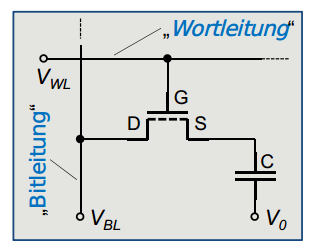
\includegraphics[width=\linewidth]{Refresh_Reason.png}
\end{center}
\begin{description}
	\item [Ursache]
	Zwischen S (Source) und D (Drain) kommt es aufgrund von Verunreinigungen zum Stromfluss.
	Ein gespeicherter Wert in C kann dadurch ungewollt abfliessen (oder sich auffüllen).
	\item[Ablauf Refresh]
	Bei einem Refresh, der alle paar 100 ns passiert, wird jeder Wert gelesen und gleich wieder geschrieben. Auf diese Weise ist die Ladung (oder nicht-Ladung) ständig in ihrer Position gehalten. Es ist gewissermassen so, als hätte man ein paar Krabbeltiere in einem offenen Glas und würde ständig die, die flüchten, wieder zurückschieben, oder die, die ungewollt hinein kriechen, wieder entfernen. 
\end{description}
Anmerkung: Skizze aus Skript entlehnt.
\end{solutionordottedlines}

	\end{questions}
\end{document}